\documentclass[a4paper,12pt]{article}

\usepackage[utf8]{inputenc}
\usepackage[T1]{fontenc}
\usepackage[polish]{babel}
\usepackage{amsmath, amssymb}
\usepackage{graphicx}
\usepackage{float}
\usepackage{hyperref}
\usepackage{geometry}
\usepackage{csvsimple} 

\geometry{margin=2.5cm}

\title{Sprawozdanie 1 z Statystyki i Modeli Liniowych}
\author{Wiktor Zoga}
\date{\today}

\begin{document}

\maketitle
\newpage

\section{Zadanie 1 - Porównywanie estymatorów}

\subsection{Opis eksperymentu}
W tym zadaniu dla kolejnych parametrów

\begin{enumerate}
    \item $\theta = 0$, $\sigma = 1$
    \item $\theta = 0$, $\sigma = 2$
    \item $\theta = 4$, $\sigma = 1$
    \item $\theta = 4$, $\sigma = 2$
\end{enumerate}

wygenerowano próby o rozmiarze $n=50$ z rozkładów: $ N(\theta, \sigma^2), Logist(\theta, \sigma), Cauchy(\theta, \sigma)$.

Dla każdej próbki obliczono dwa estymatory:

\begin{itemize}
    \item $\hat{\theta}_1$ -- średnia arytmetyczna
    \item $\hat{\theta}_2$ -- mediana
\end{itemize}

Doświadczenie powtórzono $10{,}000$ razy dla każdego zestawu parametrów i rozkładu.

\newpage

\section{Wyniki - wykresy pudełkowe i tabele statystyk}

% --- makro do wstawienia wykresu i tabeli CSV pod nim
\newcommand{\plotwithstats}[3]{
    \subsection{$\theta=#1$, $\sigma=#2$}
    \begin{figure}[H]
        \centering
        \includegraphics[width=0.9\textwidth]{../plots/boxplot_all_theta#1_sigma#2.png}
        \caption{Boxplot wszystkich rozkładów i estymatorów}
    \end{figure}

    \begin{figure}[H]
        \centering
        \includegraphics[width=0.9\textwidth]{../plots/boxplot_no_cauchy_theta#1_sigma#2.png}
        \caption{Boxplot bez rozkładu cauchy'ego}
    \end{figure}

    \begin{center}
        \csvreader[
            tabular=|l|c|c|c|c|,
            table head=\hline Estymator & Średnia & Wariancja & Bias & MSE \\ \hline,
            late after line=\\\hline,
            filter expr={true},  % brak filtrowania
            respect percent
        ]{../plots/table_theta#1_sigma#2.csv}{Estimator=\est,Mean=\mean,Variance=\var,Bias=\bias,MSE=\mse}
    {\est & \pgfmathprintnumber{\mean} & \pgfmathprintnumber{\var} & \pgfmathprintnumber{\bias} & \pgfmathprintnumber{\mse} }
    \end{center}

    \newpage
}

% --- teraz wywołanie dla wszystkich kombinacji parametrów

\plotwithstats{0}{1}

\plotwithstats{0}{2}

\plotwithstats{4}{1}

\plotwithstats{4}{2}

\subsection{Dyskusja}
\subsection*{Charakterystyka badanych rozkładów}

W zadaniu analizowane są trzy rozkłady prawdopodobieństwa, wszystkie należące do rodziny rozkładów symetrycznych,
ale o fundamentalnie różnych właściwościach (szczególnie dotyczących tzw. "grubości ogonów").

\begin{itemize}
    \item \textbf{Rozkład Normalny (Gaussa) $\mathcal{N}(\theta, \sigma^2)$}
    Jego funkcja gęstości prawdopodobieństwa (PDF) dana jest wzorem:
    \[ f(x; \theta, \sigma^2) = \frac{1}{\sigma\sqrt{2\pi}} \exp\left(-\frac{(x-\theta)^2}{2\sigma^2}\right) \]
    \begin{itemize}
        \item $\theta$: Parametr położenia. Jest to jednocześnie \textbf{wartość oczekiwana}, \textbf{mediana} oraz \textbf{dominanta} rozkładu. $E[X] = \theta$.
        \item $\sigma^2$: Parametr skali. Jest to \textbf{wariancja} rozkładu.
    \end{itemize}
    
    \item \textbf{Rozkład Logistyczny $\text{Logist}(\theta, \sigma)$}
    Rozkład symetryczny, podobny kształtem do normalnego, ale o "grubszych ogonach". Jego PDF to:
    \[ f(x; \theta, \sigma) = \frac{\exp\left(-\frac{x-\theta}{\sigma}\right)}{\sigma\left(1 + \exp\left(-\frac{x-\theta}{\sigma}\right)\right)^2} \]
    \begin{itemize}
        \item $\theta$: Parametr położenia. Podobnie jak w rozkładzie normalnym, jest to \textbf{wartość oczekiwana}, \textbf{mediana} i \textbf{dominanta}. $E[X] = \theta$.
        \item $\sigma$: Parametr skali. Nie jest to odchylenie standardowe. Wariancja tego rozkładu jest skończona i wynosi $\text{Var}(X) = \frac{\sigma^2 \pi^2}{3}$.
    \end{itemize}

    \item \textbf{Rozkład Cauchy'ego $\text{Cauchy}(\theta, \sigma)$}
    Rozkład symetryczny znany z posiadania ekstremalnie "grubych ogonów". Jego PDF:
    \[ f(x; \theta, \sigma) = \frac{1}{\pi\sigma \left(1 + \left(\frac{x-\theta}{\sigma}\right)^2\right)} \]
    \begin{itemize}
        \item $\theta$: Parametr położenia. Ze względu na symetrię rozkładu, $\theta$ jest jego \textbf{medianą} oraz \textbf{dominantą}.
        \item $\sigma$: Parametr skali.
        \item \textbf{Kluczowa uwaga:} Dla rozkładu Cauchy'ego \textbf{wartość oczekiwana oraz wariancja nie istnieją}. Całka $E[|X|]$ jest rozbieżna.
    \end{itemize}
\end{itemize}

Tak wyglądają gęstości prawdopodobieństwa tych rozkładów:

\begin{figure}[H]
    \centering
    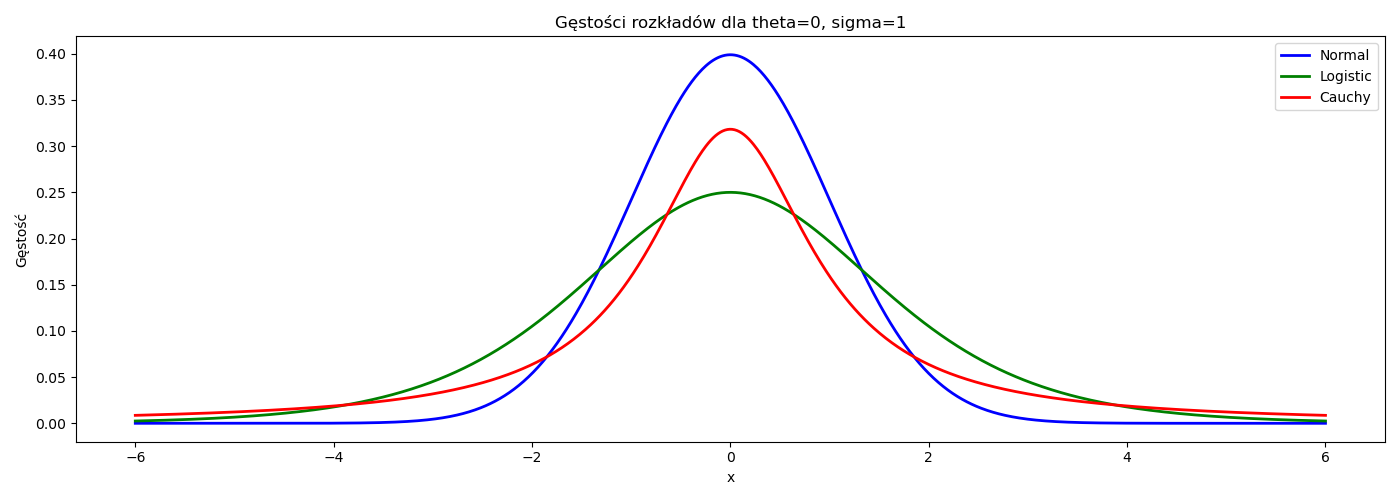
\includegraphics[width=1.0\textwidth]{../plots/theoretical_density_theta0_sigma1.png}
    \caption{Funkcje gęstości prawdopodobieństwa rozkładów Normalnego, Logistycznego i Cauchy'ego dla $\theta=0$ i $\sigma=1$}
\end{figure}

\section{Dyskusja Wyników}

Analiza porównawcza estymatorów $\hat{\theta}_1$ (średnia arytmetyczna) i $\hat{\theta}_2$ (mediana) dla trzech różnych rozkładów symetrycznych ujawnia fundamentalne różnice we właściwościach tych estymatorów.

We wszystkich trzech badanych przypadkach parametr $\theta$ pełni rolę parametru położenia, definiując \textbf{oś symetrii} funkcji gęstości.

\subsection*{Analiza Estymatora $\hat{\theta}_1$ (Średnia Arytmetyczna)}

\begin{itemize}
    \item W przypadku rozkładu \textbf{Normalnego} oraz \textbf{Logistycznego}, wartość oczekiwana istnieje i jest równa osi symetrii, tzn. $E[X] = \theta$. Dlatego w tych dwóch przypadkach średnia arytmetyczna jest nieobciążonym estymatorem parametru $\theta$, co potwierdziły wyniki symulacji (bias niski, MSE niski).

    \item Rozkład \textbf{Cauchy'ego} jest jedynym spośród badanych, który jest \textbf{pozbawiony wartości oczekiwanej}. Jest to więc estymator całkowicie nieodpowiedni do estymacji parametru położenia tego rozkładu. Wyniki symulacji odzwierciedlają tę teoretyczną katastrofę, wykazując ekstremalnie wysoką wariancję i błąd MSE.
\end{itemize}

\subsection*{Analiza Estymatora $\hat{\theta}_2$ (Mediana)}

Dla \textit{każdego} rozkładu symetrycznego, oś symetrii $\theta$ \textbf{zawsze pokrywa się z medianą} rozkładu.

Mediana z próby ($\hat{\theta}_2$) jest estymatorem mediany populacji.

Wyniki symulacji potwierdzają tę tezę. Estymator $\hat{\theta}_2$ wykazał \textbf{dobre właściwości} (niskie obciążenie i niewielki błąd MSE) dla \textbf{wszystkich trzech rozkładów}. 
Ukazuje to jego \textbf{odporność} na ekstremalnie "grube ogony" rozkładu Cauchy'ego, dla którego średnia arytmetyczna zawiodła.

\end{document}
